\begin{frame}
\frametitle{\insertsection} 
\framesubtitle{\insertsubsection}
Рассмотрим в качеству примера вызов:
\inputminted{java}{code/FlatMapFactorizeExample.java}
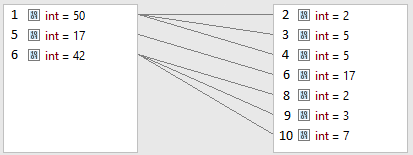
\includegraphics[scale=0.8]{img/flatMapExample.png}

Решая такие же задачи и для остальных методов, сможем получить отображения для всех. (с возможностью легко расширить набор поддерживаемых методов, например, поддержав сторонние библиотеки)
\end{frame}
